\documentclass[12pt]{article}

\usepackage[utf8]{inputenc}
\usepackage[margin=1in]{geometry}
\usepackage{graphicx}
\usepackage{caption}
\usepackage{ragged2e}
\usepackage{enumitem}
\usepackage{hanging}
\usepackage{indentfirst}
\usepackage{biblatex}
\addbibresource{final.bib}


\begin{document}
\begin{titlepage}
\vspace*{\fill}
    \begin{center}
      \huge{CS 524 - Final System Design }\\
      \vspace{40pt}
      \Large{
      Andrew Bezman - \emph{Team Lead}\\
      Nicha Unnopavong - \emph{Scrum Master}\\
      Karishma Gouni\\
      Jose Susairaj\\
      Ekene Okoroafor\\
      Christopher Smalls\\
      John Caruthers\\
      \vspace{40pt}
      December 12, 2022}
    \end{center}
    \vspace*{\fill}
\end{titlepage}


\centering
\thispagestyle{empty}
\Large{Outline and Team Member Assignments:}\\
\vspace{1em}
\begin{enumerate}[label*=\arabic*.]
\normalsize
    \item System Description \emph{(All)}
        \begin{enumerate}[label*=\arabic*.]
            \item Description and Diagram
            \item Platform and System Requirements
            \item Technology Stack
        \end{enumerate}
    \item Components
        \begin{enumerate}[label*=\arabic*.]
            \item Logon Page \emph{(Ekene)}
            \item Communicator \emph{(Nicha, Karishma)}
            \item Learning Center \emph{(Jose, Andrew, Christopher)}
            \item Database \emph{(Andrew, John)}
        \end{enumerate}
    \item Games
        \begin{enumerate}[label*=\arabic*.]
            \item Game 1 \emph{(Andrew)}
            \item Astronaut Quiz \emph{(Karishma)}
            \item Space Quiz \emph{(Jose)}
            \item Game 4 \emph{(Ekene)}
            \item Sliding Puzzle \emph{(Nicha)}
            \item Problem-Solving \emph{(Christopher)}
            \item Math Defense \emph{(John)}
        \end{enumerate}
    \item References
\end{enumerate}

\pagebreak
\normalsize
\setcounter{page}{1}
\justify

\section{System Description}
    \subsection{Description and Diagram}

    Our Astronaut Training Application is a web based application that can be run on most browsers from a computer or mobile device.  The goal of our Astronaut Training Application is to provide a space-themed, fun and educational, resource for adults and children who are interested in astronomy, physics, mathematics, and the history of discovery in outer space. It does this by using space based games to educate the players.  Players are able to make an account and track their progress.  Games are meant to be quick games that can be completed in 5 minutes or less.

    \begin{figure}[ht]
        \centering
            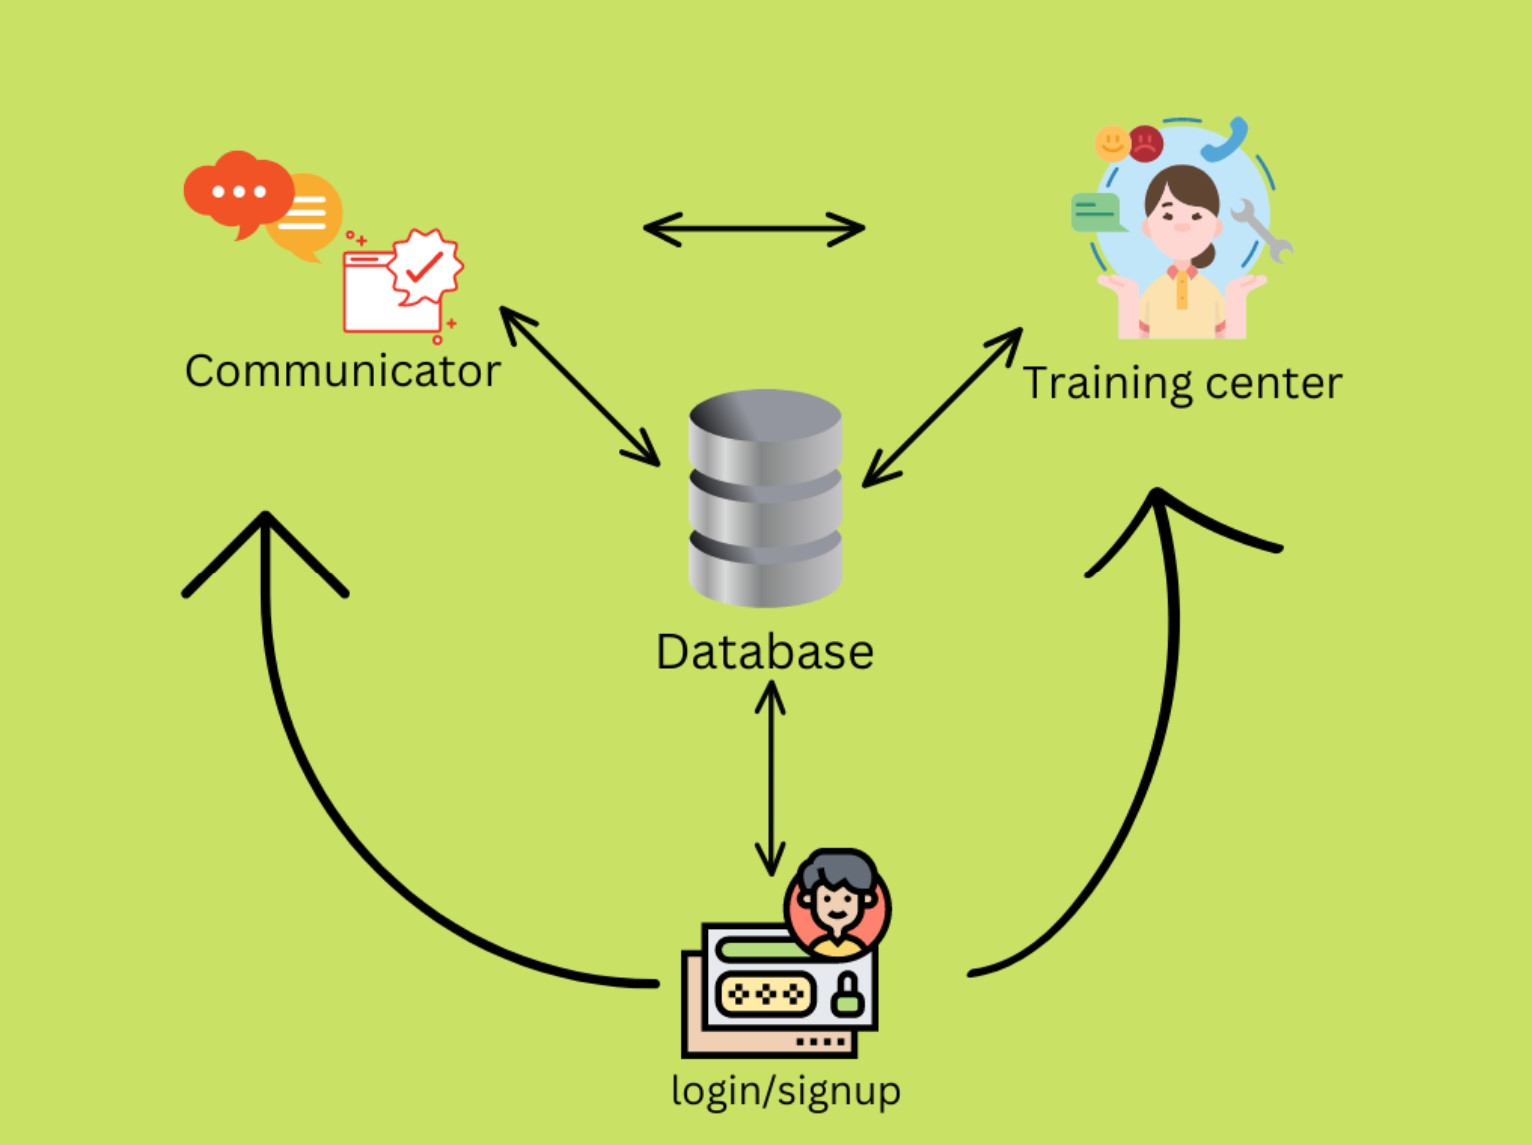
\includegraphics[height=0.3\textheight]{ComponentDiagram.jpg}
            \caption{Component Diagram}
    \end{figure}
    
    Components of the application are the Logon Page, Communicator, Learning Center and Database.  Figure 1 above shows how these components interact.  First, players will create an account on the Logon Page.  This data is stored on the client's device.  Once an account is made, the player is directed to the Learning Center where they are able to see their progress and can click on buttons to play games. The Communicator emails the players when they make an account, and of any progress they have made.  It will also remind players of daily challenges.

    The component diagram above shows how the components interact with one another.  The login/signup page will write data to the database when a new player signs up.  For login, the database is used to verify the correct data, returning a boolean value to the login.  The login/signup also page will direct players to the Training Center after a successful login.  The training center interacts with the database to write score updates after the player completes a game.  It will also send data to the communicator to congratulate user for completing a game. The communicator reads data from the database for emailing users.  

    \subsection{Platform and System Requirements}

    The Astronaut Training Application is meant to run on internet browsers on a computer or mobile device.  It is hosted on AWS Amplify and utilizes Amazon Web Services (AWS) Lambda functions to provide intractability between the different components and games.  The players data is not stored on the server, it is stored on the clients local storage of the player's browser utilizing Mozilla Client Side Storage.  The user can use Chrome, Edge or Firefox on either Windows, Linux or iOS.  Any browser that is compatible with JavaScript ES5 and above is suitable to run this application.
    
    \subsection{Technology Stack}

    Many tools were used to build the visual content of this application.  These include: InkScape, Adobe Illustrator, Adobe Photoshop, Figma, Paint, Tiled, and Canva. Secondly, content was made with HTML, CSS and JavaScript.  Program logic was built with JavaScript.  There are two sections to the database: Mozilla Client Side Storage, and AWS.  Username, passwords, emails and scores are stored locally on the clients device.  AWS stores the HTML, CSS and JavaScript files of all components and games.  The logic is run on the cloud using AWS Amplify, AWS API Gateway, and AWS Lambda. Figure 2 below shows the layers.

    \begin{figure}[ht]
        \centering
            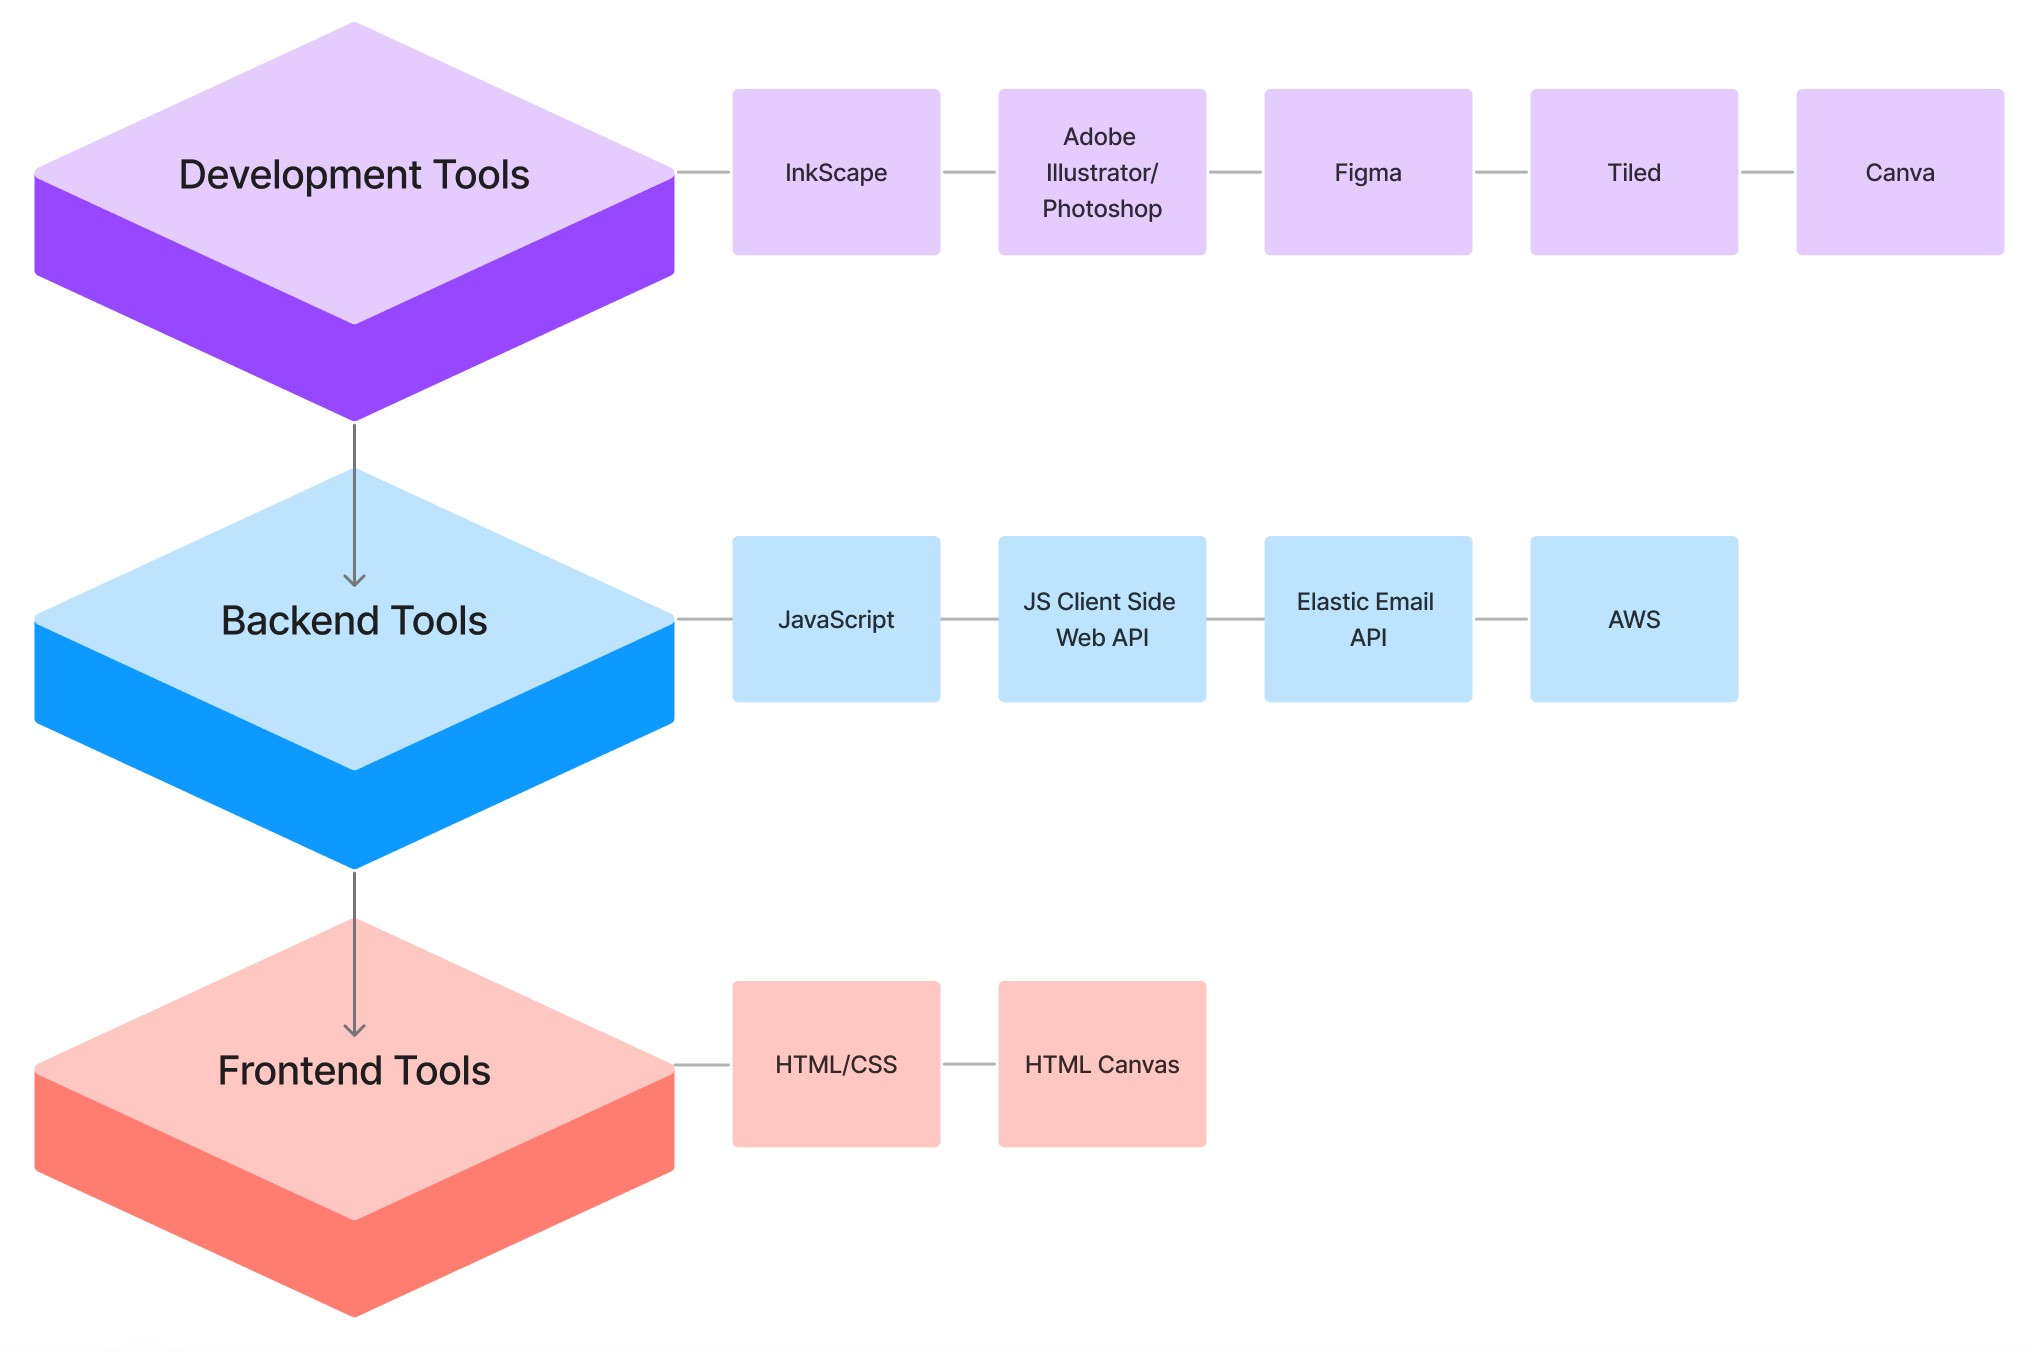
\includegraphics[height=0.4\textheight]{TechStackD.jpg}
            \caption{Technology Stack}
    \end{figure}

\section{Components}
    \subsection{Logon Page}

    Insert Text

    \subsection{Communicator}

    The communicator works on the client’s device and communicates with them via email and notifications that relate to our web app. SMTP server handles sending email automatically, once clients have signed up. The "Today’s challenges" will be reminded by notifications. Communicator validates the email and passwords of the user. In case of invalid details, it shows a popup.\cite{smtp}

    \subsection{Learning Center}
    The learning center and training center were combined to the Learning Center.  Chris worked on the training center application and Jose/Andrew worked on the learning center application.  The Learning Center is a home screen for the user.  A user interface that displays the user's profile, scores, and progress towards completion. Also, buttons that take them to a game of whichever type is titled on the button. (Chris) The learning center contains the demo video for the application. Along with the tutorial video it also acts as a platform for various articles, recent events and study materials for the users to enhance the knowledge on Astronomy and Space. (Jose)

    \begin{figure}[ht]
        \centering
        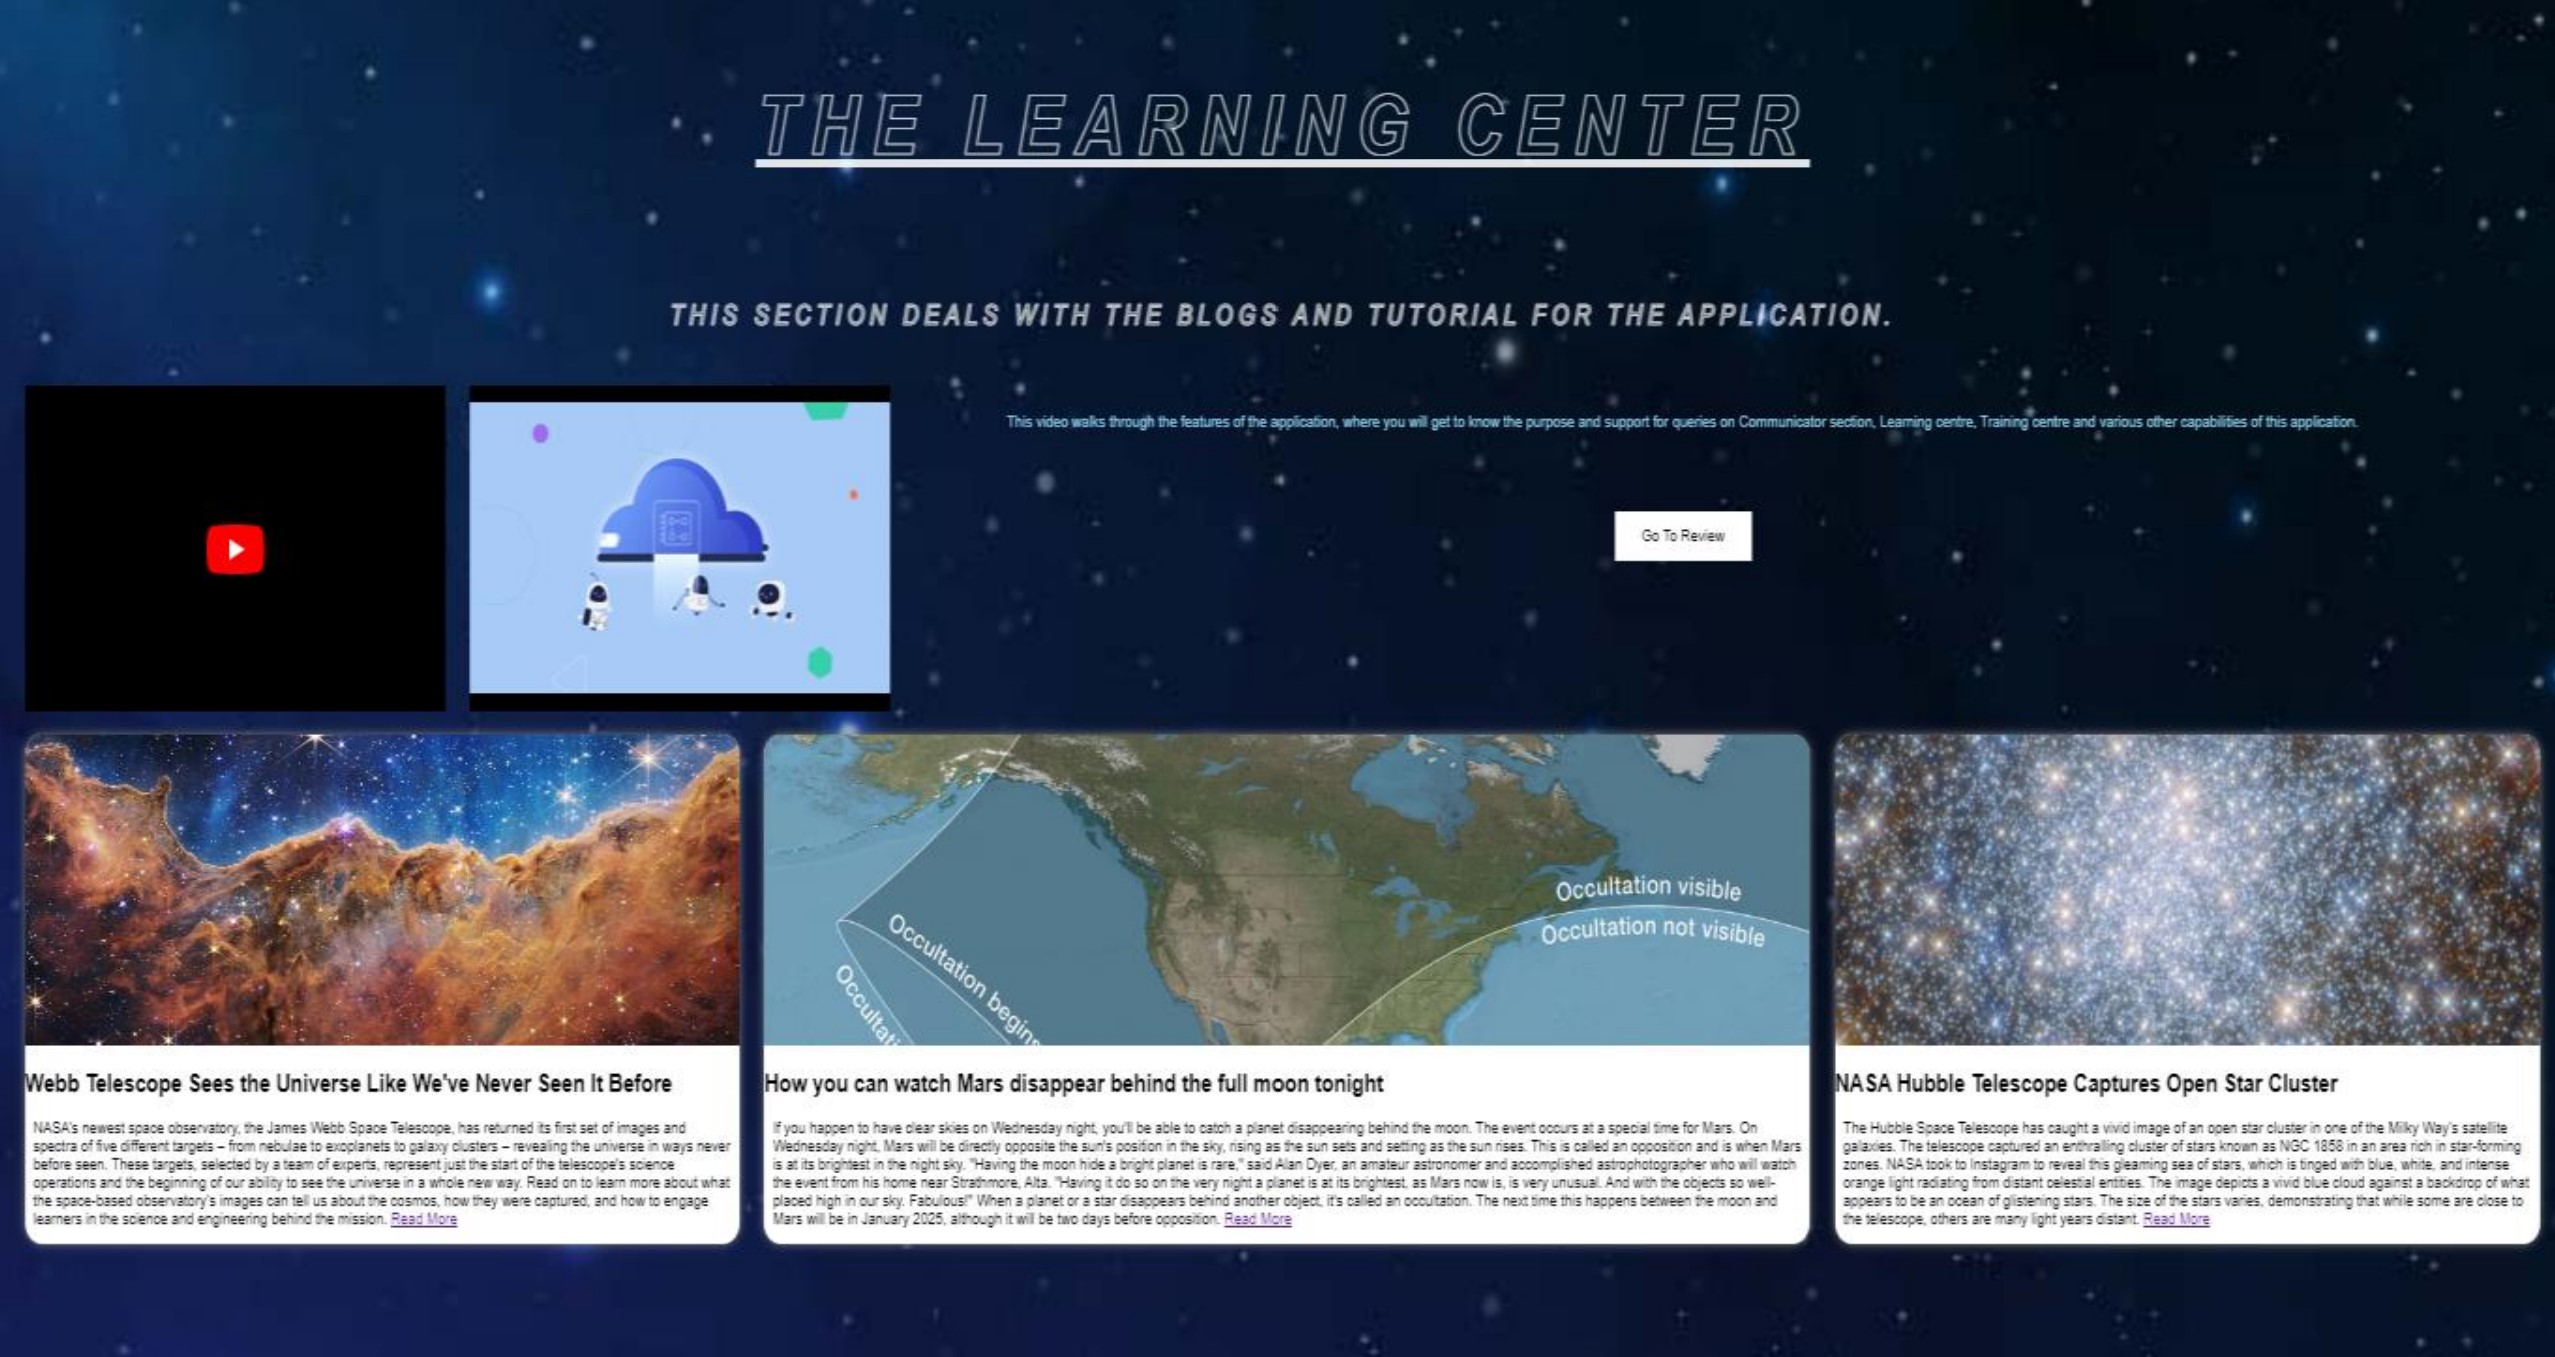
\includegraphics[height=0.35\textheight]{LearningCenter.jpg}
        \caption{Learning Center}
    \end{figure}

    \subsection{Database}
    The database is broken up into two components.  First the client's browser stores the player's username, email, password, and scores.  Next, AWS hosts the website and stores the HTML, CSS, and JavaScript files.  All logic is performed in the cloud using AWS Amplify, AWS Lambda and AWS API Gateway\cite{MozCS}\cite{AWS}.

\section{Games}
    \subsection{Game 1}

    Insert Text

    \newpage
    
    \subsection{Astronaut Quiz}

    Astronaut quiz is a fun game which trials the players knowledge.  This game consists of questions related to the life of an astronaut in space, and interesting facts about space and the universe. This game will have 10 questions and each right attempt increases the score to 100 points. Every question will have a hint, which helps to solve the quiz with more comfort.

    \begin{figure}[ht]
        \centering
            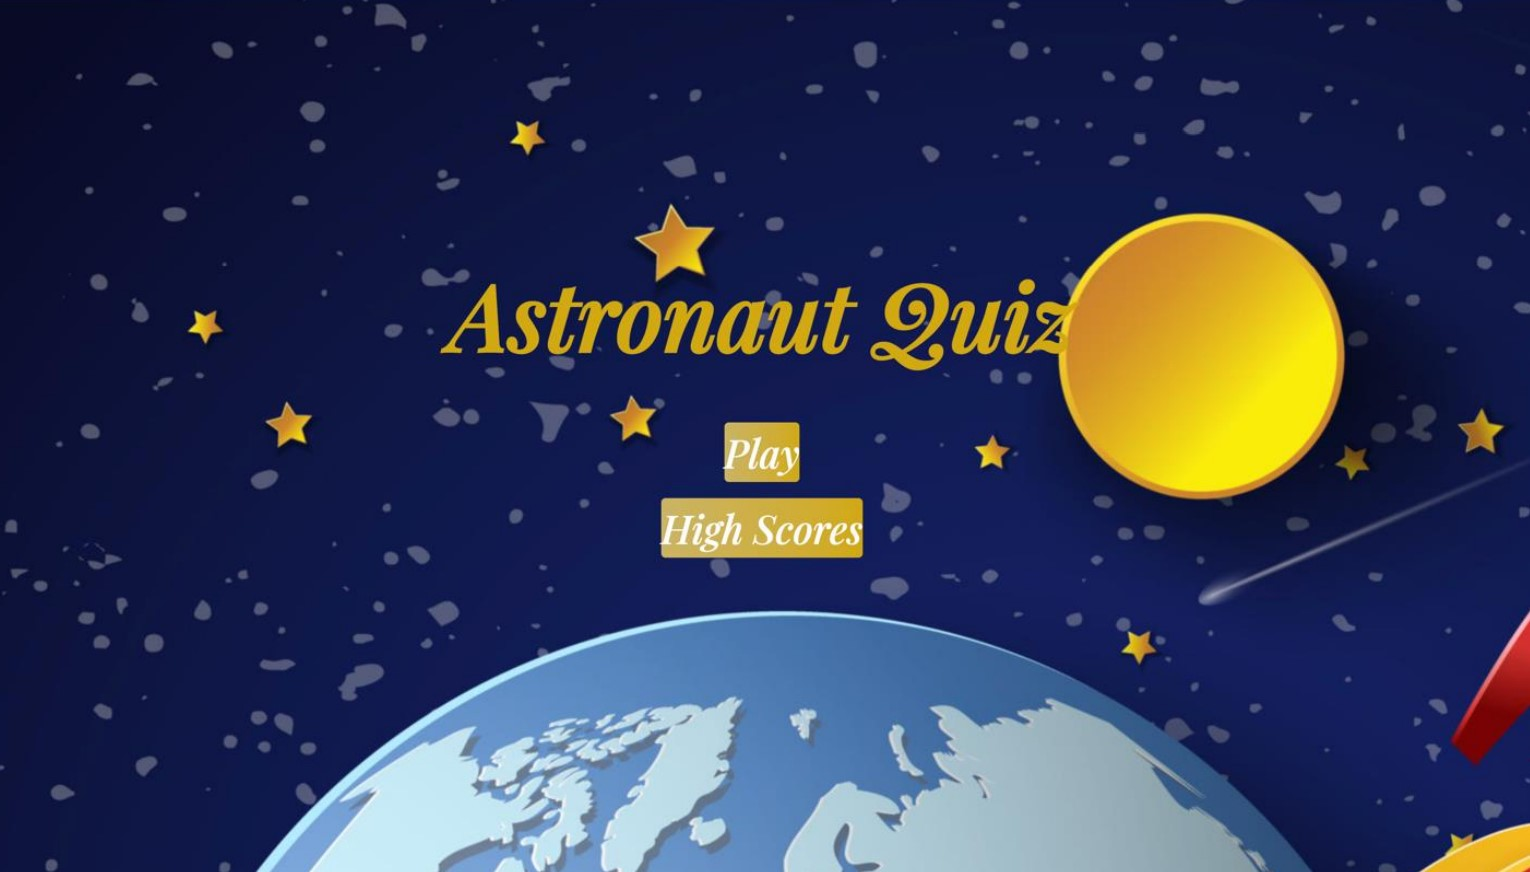
\includegraphics[height=0.3\textheight]{quizGameK1.jpg}
            \caption{Astronaut Quiz Into Page}
    \end{figure}

    \begin{figure}[ht]
        \centering
            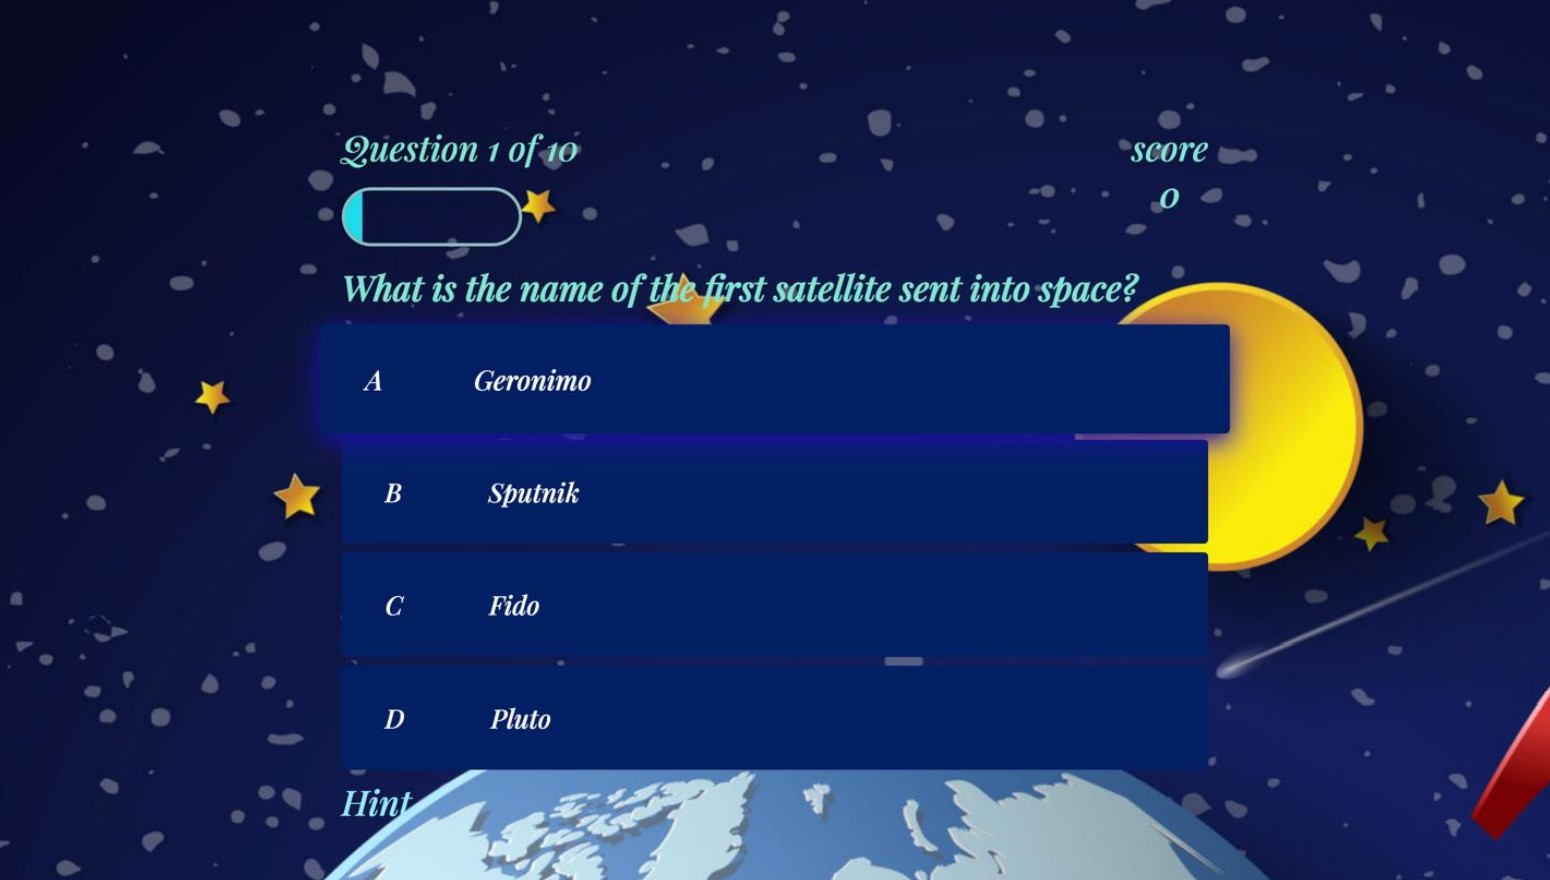
\includegraphics[height=0.3\textheight]{quizGameK2.jpg}
            \caption{Astronaut Quiz Question Example}
    \end{figure}
    
    \newpage

    \subsection{Space Quiz}

    The quiz game enables users to answer 10 random questions with 4 options. Once the user finished answering the 10 questions, the result score is calculated and both right and wrong answers are displayed for a better understanding to the user.

    \begin{figure}[ht]
        \centering
            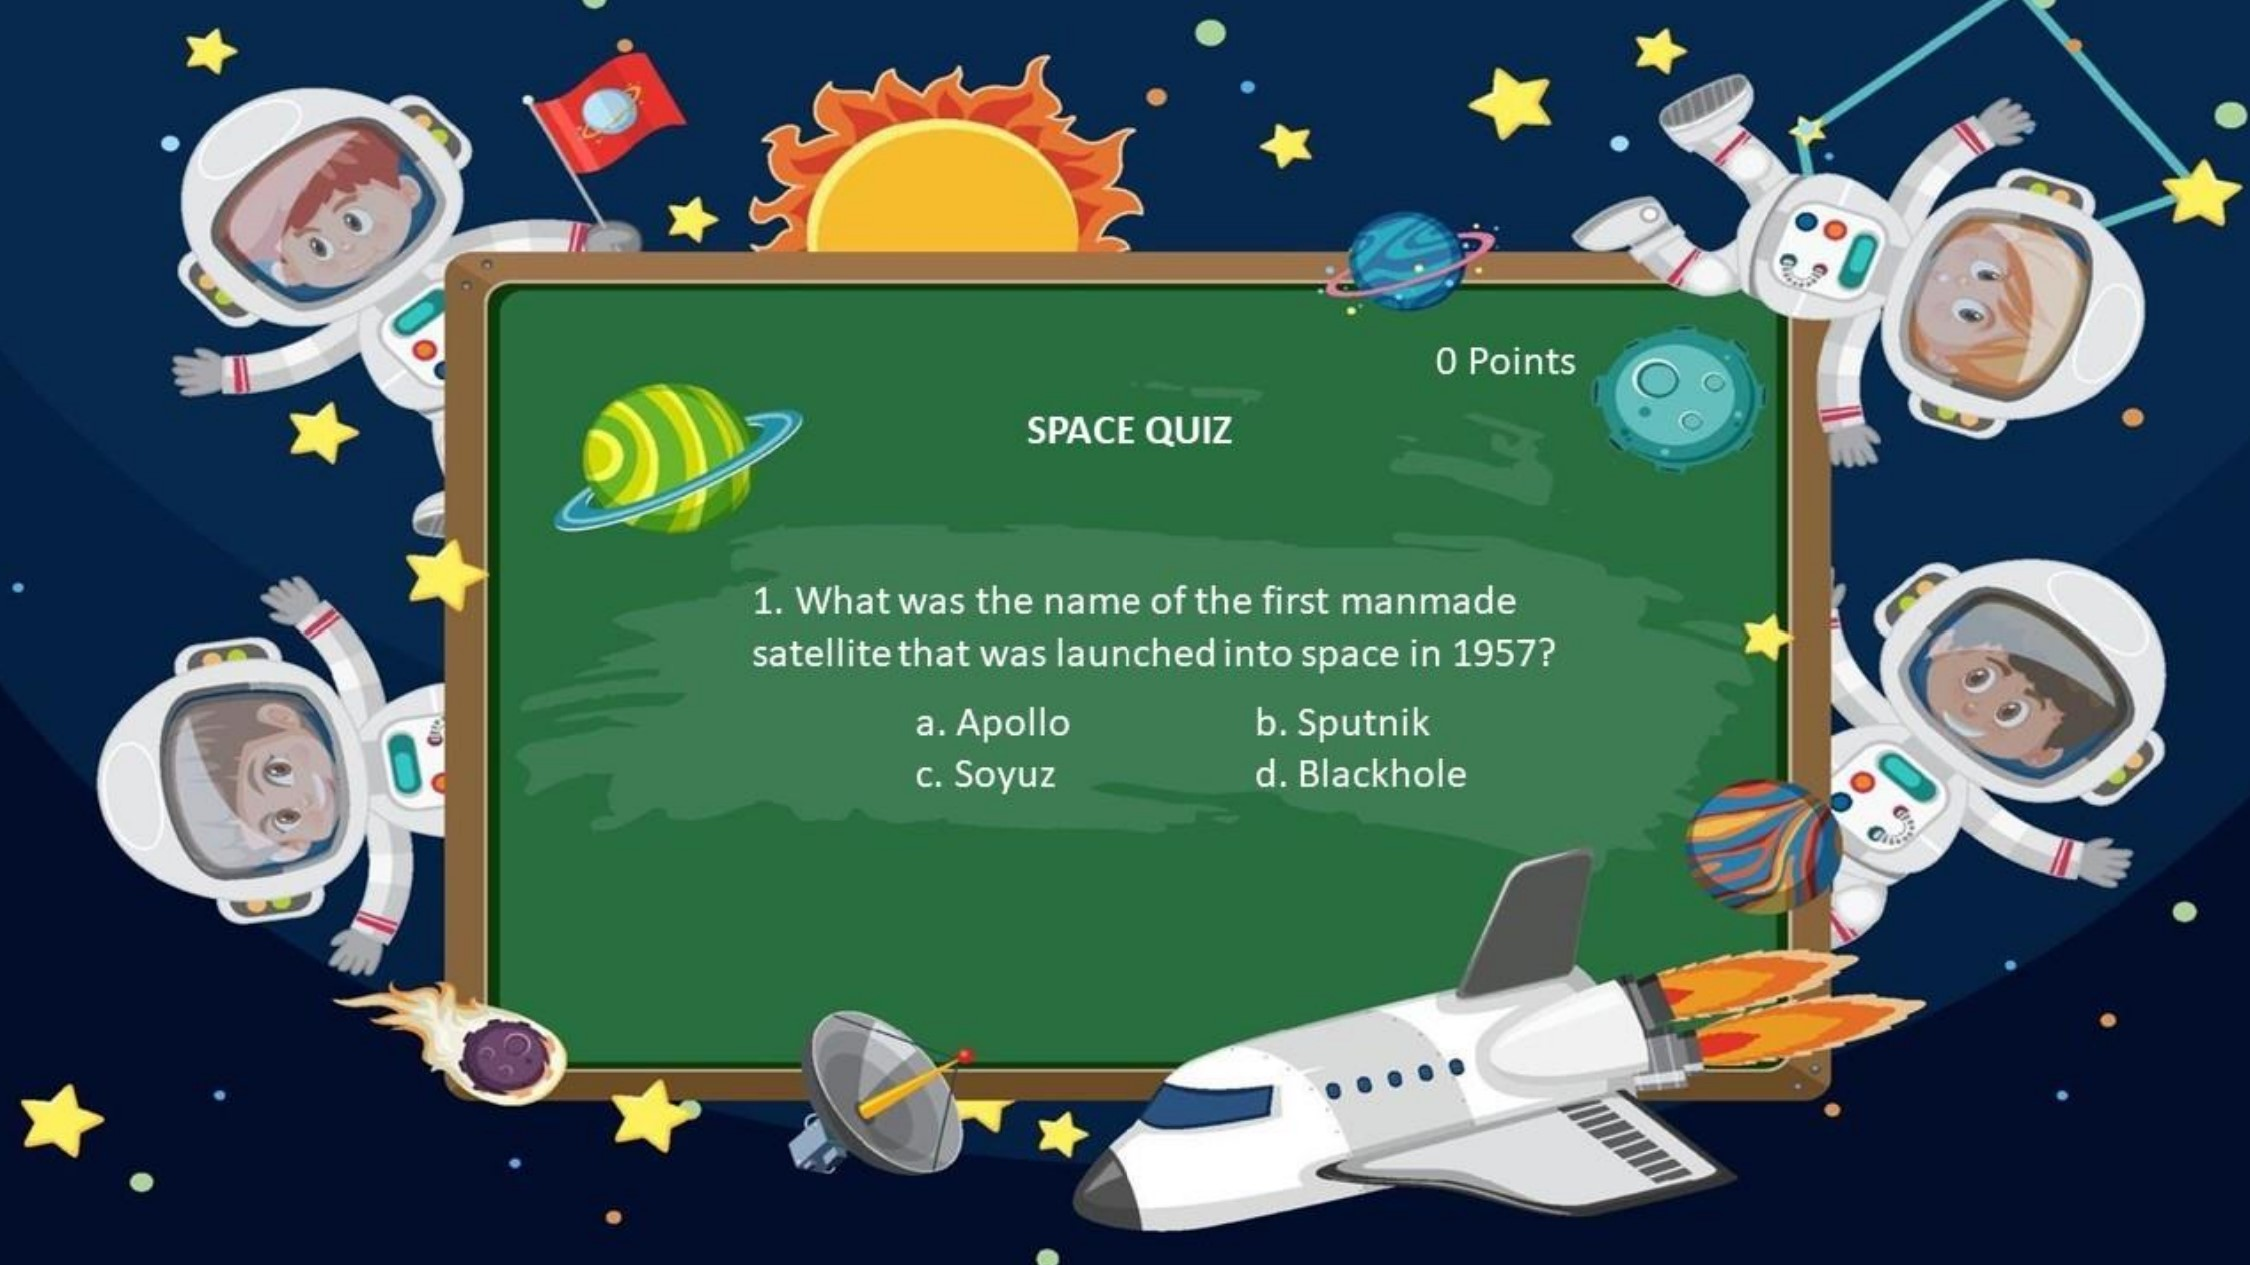
\includegraphics[height=0.3\textheight]{spacequiz.jpg}
            \caption{Space Quiz Snip}
    \end{figure}

    \subsection{Game 4}

    Insert Text

    \subsection{Sliding Puzzle}

    A sliding puzzle game is a problem-solving game in which the player has to slide the tiles around the board until the tiles have been arranged in the correct order. By dragging the pieces in want to move to the empty space beside it. The challenge is how to finish the game in a minimum number of moves.

    \subsection{Problem-Solving}
    A memory matching game that enables a user to select a card and attempt to find the card that has a similar graphic. When the user clicks a button titled problem-solving, a list of games is displayed which contains the game.  
    
    \newpage

    \subsection{Math Defense}

    Math Defense is a space based tower defense game that has the player build defenses to protect the moon base from alien attackers.  The player generates income for tower purchases by solving math problems.  Math problems are simple addition, subtraction and multiplication problems. Each enemy wave becomes increasingly harder and includes more enemies.  The enemies become faster and more numerous as each wave progresses.   The game ends when the moon base health reaches 0. The figure below shows a snip of the Math Defense game.  Red circles are enemies, dark blue squares are defense towers, light grey squares (around the path) are areas where towers can be built.  The HUD shows the wave number, currency and health.  Below the canvas is the math puzzle with multiple choice answers\cite{MozJS}\cite{RMO}\cite{CanCC}.
    \begin{figure}[ht]
        \centering
            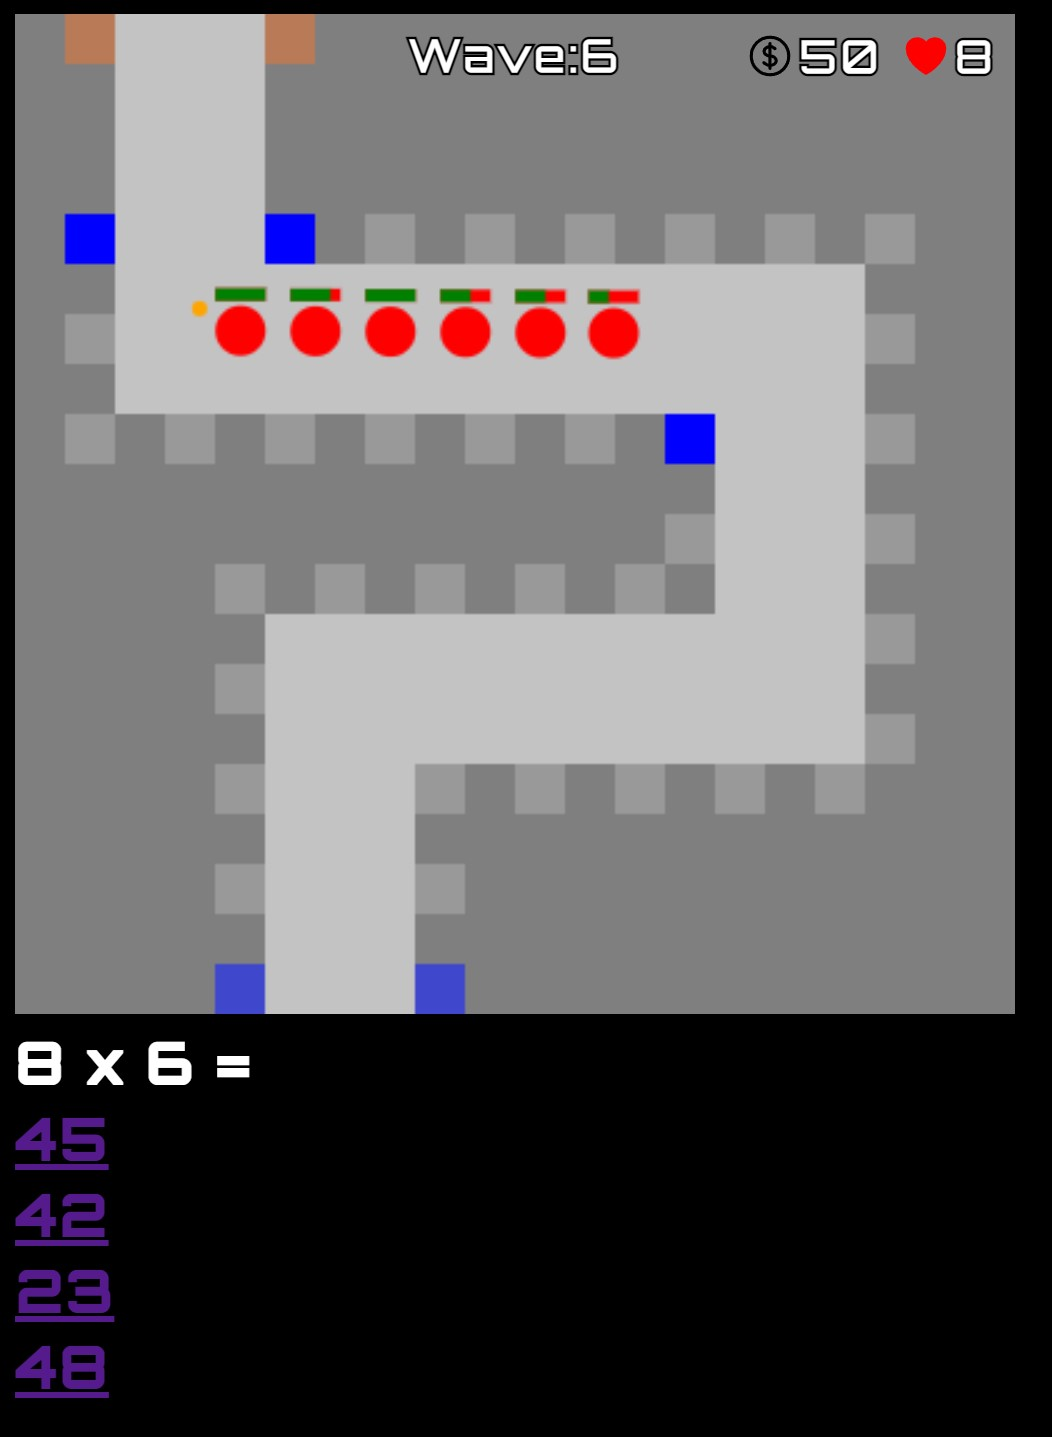
\includegraphics[height=0.30\textheight]{mathDefenseSnip.jpg}
            \caption{Math Defense Snip}
    \end{figure}

\newpage
\printbibliography
\end{document}
